% --- Dokumententyp ---
% Dokumententyp scrreprt; deutsch, doppelseitig mit 1cm Bindekorrektur
\documentclass[BCOR=1cm, ngerman]{scrreprt}

% --- Präambel ---
% Erweiterungen einbinden
\usepackage[utf8]{inputenc}
\usepackage{babel}
\usepackage[backend=biber]{biblatex}
\usepackage{amsmath}
% für hyperlinks:
\usepackage{hyperref}
\hypersetup{
  hidelinks,
  colorlinks=false}
\usepackage{cleveref}
\usepackage[multiple]{footmisc}
\usepackage{graphicx}
\graphicspath{{imgs/}}
\usepackage{csquotes}

% um zeilenumbrüche in Tabellen zu erstellen
\usepackage{makecell}

% für subfigure:
\usepackage{caption}
\usepackage{subcaption}

% tikz pakete für die Erstellung von plots:
\usepackage{tikz}
\usepackage{tikz-timing} % für timing-diagramme:
\usepackage{pgfplots}
\pgfplotsset{compat=newest}
% für svg bilder:
\usepackage{svg}

% formatierung von code im text:
\newcommand{\code}[1]{\texttt{#1}}
% formatierung von bit vektoren, digitalen werten und analogen Werten
\newcommand{\bit}[1]{\code{#1}}
\newcommand{\bitvect}[1]{\code{#1}}
\newcommand{\analog}[1]{\code{#1}}
% low-activ Signal:
\newcommand{\lowactive}[1]{$\overline{\bit{#1}}$}

% Attribute für die Titelseite
\titlehead{\hfill
\includegraphics[width=4cm]{logo.png}} % Das FH-Logo
\subject{Fachhochschule Bielefeld\\Fachbereich Ingenieurwissenschaften und Mathematik\\Studiengang Ingenieurinformatik}
\title{Entwicklung und Implementierung eines digitalen Funktionsgenerators in VHDL}
\subtitle{Studienarbeit}
\author{Markus Hartlage 1103528}
\date{\today} % Das Datum der Abgabe
\publishers{Betreuer:\\ Prof. Dr. Axel Schneider\\Dr. Hanno Gerd Meyer\\Kevin Hunke}

% Pfad zur bib-Datei mit Literaturquellen
\bibliography{references.bib}
\addbibresource{references.bib}

% --- Dokumentenrumpf ---
\begin{document}
% Titelseite erstellen
\maketitle

% Deutsche und englische Zusammenfassung in abstract-Umgebung
\begin{abstract}
  In dieser Studienarbeit wird die Implementation eines Funktionsgenerators mithilfe der Hardwarebeschreibungssprache VHDL geschildert.
  Der Aufbau des Generators wird erläutert sowie seine korrekte Funktion überprüft.
  Darüber hinaus werden seine Leistungsdaten erfasst und dargelegt.
  Die Ergebnisse der Arbeit zeigen, dass der Generator zuverlässig in einem Frequenzbereich von 0,1 Hz bis 10 kHz und einem Spannungsbereich von 0 bis 3,2 V funktioniert.
  Über 10 kHz hinaus weist er Abweichungen zwischen gewünschtem und tatsächlichem Funktionsverlauf auf.
  Abweichungen treten in diesem Frequenzbereich auch zwischen der Soll- und Ist-Frequenz auf.
  Diese können nur teilweise erklärt werden, weshalb weitere Untersuchungen nötig sind, um den Frequenzbereich des Generators ganz ausschöpfen zu können. \\
  Außerdem wurde die UART-Schnittstelle getestet, mit der der Generator konfiguriert werden kann.
  Dieser Test verlief erfolgreich. Die Befehle zur Konfiguration und ihre Funktion werden ebenfalls dokumentiert. \\
  Sämtlicher Quellcode findet sich in einem GitHub-Repository unter folgender URL: \\
  \href{https://github.com/markushart/studienarbeit_function_generator.git}{\code{https://github.com/markushart/studienarbeit\_function\_generator.git}}
  \\

  This student research project documents the implementation of a function generator using the hardware description language VHDL.
  The composition of the generator is explained and its correct function is checked.
  In addition, its performance data is recorded and presented.
  The results of this research shows, that the generator operates reliably in a frequency range of 0,1 Hz to 10 kHz and a voltage range of 0 to 3,2 V.
  Beyond 10 kHz, it exhibits deviations between desired and actual operation.
  Deviations also occur between the desired and actual frequencies in this frequency range.
  These can only be explained partly, so further research is necessary to exhaust the full possible frequency range. \\
  In addition, the UART interface was tested, which can be used to configure the generator.
  This test was successful. The commands for configuration and their function are also documented. \\
  All source code can be found in a GitHub repository at the following URL: \\
  \href{https://github.com/markushart/studienarbeit_function_generator.git}{\code{https://github.com/markushart/studienarbeit\_function\_generator.git}}
  \\

\end{abstract}

% Erstelle Inhaltsverzeichnis
\tableofcontents
% Quellenverzeichnis setzen, welches im Inhaltsverzeichnis als Kapitel erscheinen soll. Der Titel soll 'Literaturverzeichnis' sein.
\printbibliography[heading=bibintoc, title={Literaturverzeichnis}]


% Einleitung
\chapter[Einleitung]{Einleitung}

Diese Studienarbeit behandelt die Konzipierung und Implementierung eines digitalen Funktionsgenerators in der Hardwarebeschreibungssprache VHDL.
Ein Funktionsgenerator ist ein elektronisches Bauteil, das in der Lage ist, verschiedene Spannungsverläufe an seinem Ausgang auszugeben.
Diese können dann an andere Bauteile angeschlossen und so technisch genutzt werden.
Beispielsweise kann ein Funktionsgenerator eingesetzt werden, um ein Rechteck- oder Sinussignal auszugeben.
Der praktische Nutzen könnte dann die Aktivierung eines Kameraauslösers in einer bestimmten Frequenz oder die Helligkeitssteuerung einer LED sein. \\
Ein Funtkionsgenerator kann als Digitalschaltung in einen Chip integriert oder auf eine Platine gelötet werden, er könnte aber auch als Programm eines Universalrechners laufen.
Softwarelösungen verfügen nicht über das hohe Maß an Effizienz und die Geschwindigkeit einer integrierten Schaltung.
Diese wiederum sind nur in großer Stückzahl rentabel herstellbar.
Von Hand gelötete Schaltungen lassen sich nicht einfach reproduzieren und sind nicht besonders kompakt.
Einen Mittelweg zwischen diesen Zielkonflikten bieten sogenannte ``\textbf{F}ree \textbf{P}rogrammable \textbf{G}ate \textbf{A}rrays'', kurz FPGA.
Auf diesen ICs befinden sich verschiedene Bausteine die durch Anlegen einer Programmierspannung miteinander verknüpft werden können.
Somit ist es möglich, verschiedenste Schaltungen auf demselben IC umzusetzen. \\
Die Schaltungen können mithilfe einer Beschreibungssprache designed werden.
Eine dieser Sprachen ist VHDL (``\textbf{V}ery \textbf{H}ighspeed Hardware \textbf{D}escription \textbf{L}anguage''), welche in dieser Studienarbeit verwendet werden soll.
Die Implementation auf einem FPGA mittels Beschreibungssprache bietet den Vorteil guter Reproduzierbarkeit bei vergleichsweise hoher Konfigurierbarkeit und Effizienz. \\
Bei dem in diesem Projekt verwendeten FPGA handelt es sich um den Artix 7 von Xilinx.
Dieser ist in das Entwicklungsboard Basys 3 des Herstellers digilent eingebettet \cite{digilent2016}.
Es verfügt über diverse Peripheriemodule wie eine UART Schnittstelle, einen micro-USB Anschluss oder einen VGA Ausgang. \\
In dieser Arbeit wird zunächst der konzeptuelle Aufbau des Funktionsgenerators erläutert, dann werden die einzelnen Komponenten, aus denen er besteht, sowie die interne Taktung der Komponenten erläutert.
Schließlich wird noch ein Funktionstest durchgeführt, bei dem die theoretisch erwarteten Resultate den tatsächlichen gegenübergestellt werden. \\
Sämtlicher Quellcode findet sich im GitHub-Repository unter folgender URL: \\
\href{https://github.com/markushart/studienarbeit_function_generator.git}{\code{https://github.com/markushart/studienarbeit\_function\_generator.git}}
% Hauptteil
\chapter{Konzept}
Im Folgenden werden die verschiedenen Funktionsmerkmal des Funktionsgenerators erläutert.
Anschließend wird sein Konzept anhand des grundlegenden Aufbaus des Funktionsgenerators erklärt.
 
\section{Funktionsmerkmale} \label{Concept:Feature}
In diesem Abschnitt wird geschildert, was der Generator leisten kann und wie er sich konfigurieren lässt. 

\subsection{Funktionen} \label{Concept:Feature:Func}
Der Generator kann auf vier verschiedene Funktionsbausteine zurückgreifen, die jeweils einen anderen Spannungsverlauf ausgeben:

\begin{enumerate}
   \item \textbf{Konstante Funktion} \\ 
    Die konstante analoge Spannung \analog{high} liegt am Ausgang an.
  \item \textbf{Rechteck-Funktion} \\
    Der Wert wechselt zwischen \analog{high} und \analog{low} in der Frequenz $f$.
    Der Anteil der Zykluszeit $T$, in dem der Ausgang auf \analog{high} ist, wird über den Parameter dutycycle eingestellt.
    Die Dauer des \analog{high}-Pegels bzw. \analog{low}-Pegels, $T_{h}$ und $T_{l}$ berechnen sich folgendermaßen:
    \begin{align}
      T_{l} &= T \cdot \frac{dutycycle}{255}, dutycycle \in \{0, 1, ..., 255\} \label{Concept:Feature:Func:eqdc1} \\
      T_{h} &= T - T_{l} \label{Concept:Feature:Func:eqdc2}
    \end{align}
    Auf diese Art lassen sich Rechteck-Signale mit einstellbarer Pulsweite erzeugen.
    Diese sogenannten PWM-Signale (``\textbf{P}uls \textbf{W}eiten \textbf{M}odulation'') werden in vielen technischen Anwendungen verwendet.
  \item \textbf{Zick-Zack-Funktion} \\
    Der Analogwert steigt von \analog{low} bis \analog{high} linear an, erreicht er \analog{high}, fällt der Analogwert wieder kontinuierlich auf \analog{low} ab. Somit schwankt der Ausgangspegel mit der Frequenz $f$.
  \item \textbf{Rampen-Funktion} \\
    Der Analogwert wächst, wie bei der Zick-Zack-Funktion, linear bis auf \analog{high} an, danach fällt er aber auf \analog{high} zurück.
    Alternativ kann die Rampe auch von \analog{high} her abfallen und bei Erreichen von \analog{low} wieder auf \analog{high} zurück springen.
\end{enumerate}

\begin{figure}[h] \centering
  {
    \pgfplotsset{
    xtick={0, 15, 30, 45, 60, 75, 90},
    ytick={0, 0.55, 1.1, 1.65, 2.2, 2.75, 3.3},
    xmin=0, xmax=90,
    ymin=-0.2, ymax=3.5,
    % xlabel=$t$,
    xticklabels={$0$, , $T$, , $2T$, , $3T$,}, % \pgfmathprintnumber{\tick}},
    yticklabels={},
    grid=major,
    width=0.52\textwidth,
    height=0.4\textwidth}
  % constant
  \subfloat[][konstante Funktion]{ 
    \begin{tikzpicture}
      \begin{axis}[yticklabels={$h$, , , , , ,$l$}, ylabel=$U(t)$]
        \addplot[color=blue] coordinates{(0, 1.75)(90, 1.75)};
      \end{axis}
    \end{tikzpicture}
    \label{Concept:Plot:const}
  } 
  % square
  \subfloat[][Rechteckfunktion]{
    \begin{tikzpicture}
      \begin{axis}
        \addplot[color=blue]  coordinates{(0, 0)(15, 0)(15, 3.3)(30, 3.3)(30, 0)(45, 0)(45, 3.3)(60, 3.3)(60, 0)(75, 0)(75, 3.3)(90, 3.3)};
      \end{axis}
    \end{tikzpicture}
    \label{Concept:Plot:square}
  } 

  % zigzag \foreach \x in {0, 15, ..., 90} {(\x, 3.3)}
  \subfloat[][Zick-Zack-Funktion]{
    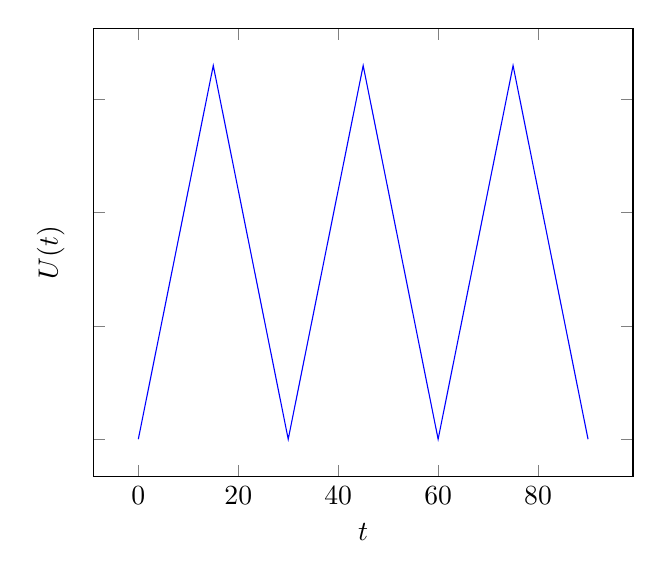
\begin{tikzpicture}
      \begin{axis}[yticklabels={$h$, , , , , ,$l$}, ylabel=$U(t)$, xlabel=$t$]
        \addplot[color=blue] coordinates{(0, 0)(15, 3.3)(30, 0)(45, 3.3)(60, 0)(75, 3.3)(90, 0)};
      \end{axis}
    \end{tikzpicture}
    \label{Concept:Plot:zigzag}
  }
  % ramp
  \subfloat[][Rampenfunktion]{
    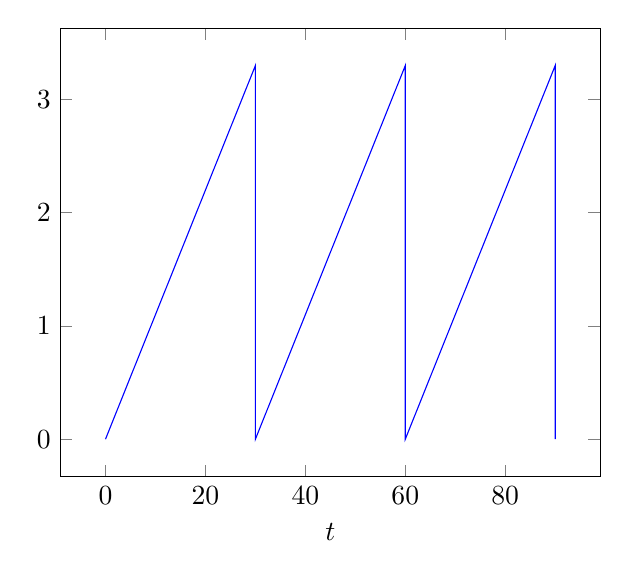
\begin{tikzpicture}
      \begin{axis}[xlabel=$t$]
        \addplot[color=blue, domain=0:90]  coordinates{(0, 0)(30, 3.3)(30, 0)(60, 3.3)(60, 0)(90, 3.3)(90, 0)};
      \end{axis}
    \end{tikzpicture}
    \label{Concept:Plot:ramp}
  }
  \caption{Funktionen, die der Funktionsgenerator ausgeben kann. Ihr Verlauf ist als Spannung $U(t)$ über der Zeit $t$ aufgetragen. Die Zykluszeit und \analog{high} bzw. \analog{low} sind durch  $T$, $h$ und $l$ gekennzeichnet.} \label{Concept:Plot}
\end{figure}

\subsection{Konfiguration}
Der Funktionsgenerator muss, um extern konfiguriert werden zu können, über eine Möglichkeit für Nutzereingaben verfügen.
Zu diesem Zweck wird die UART-Schnittstelle auf dem Basys 3-Board genutzt.
Über diese kann der Nutzer Konfigurationsbefehle per Computer versenden, die dann vom Generator interpretiert werden.
Darüber hinaus nutzerseitig wurde ein Python-Script geschrieben, das die Kommunikation mit dem Generator vereinfacht.

\section{Aufbau}
Der Funktionsgenerator ist aus verschiedenen Einzelkomponenten zusammengesetzt.
Ihre Verschaltung im Generator ist in \cref{Concept:FuncGenDia} zu sehen.
In der Abbildung kann man gut erkennen, dass die verschiedenen Funktionen parallel arbeiten und von der Konfigurationsschnittstelle mit den Signalen \bitvect{cyc\_ticks}, \bitvect{high}, \bitvect{low}, \bitvect{thresh} und \bitvect{direction} gesteuert werden.
Das Signal \bitvect{waveform} steuert den Multiplexer, der das Ausgabesignal \bitvect{y\_out} an die interne Schnittstelle des DAC-Wandlers weitergibt.
Diese Schnittstelle generiert daraus die Signale \lowactive{SYNC}, \bit{DINA}, \bit{DINB} und \bit{CLK} und transferiert sie dann an den DAC-Wandler.
Dieser wandelt sie anschließend in ein analoges Signal um.

\begin{figure}[h] \centering
  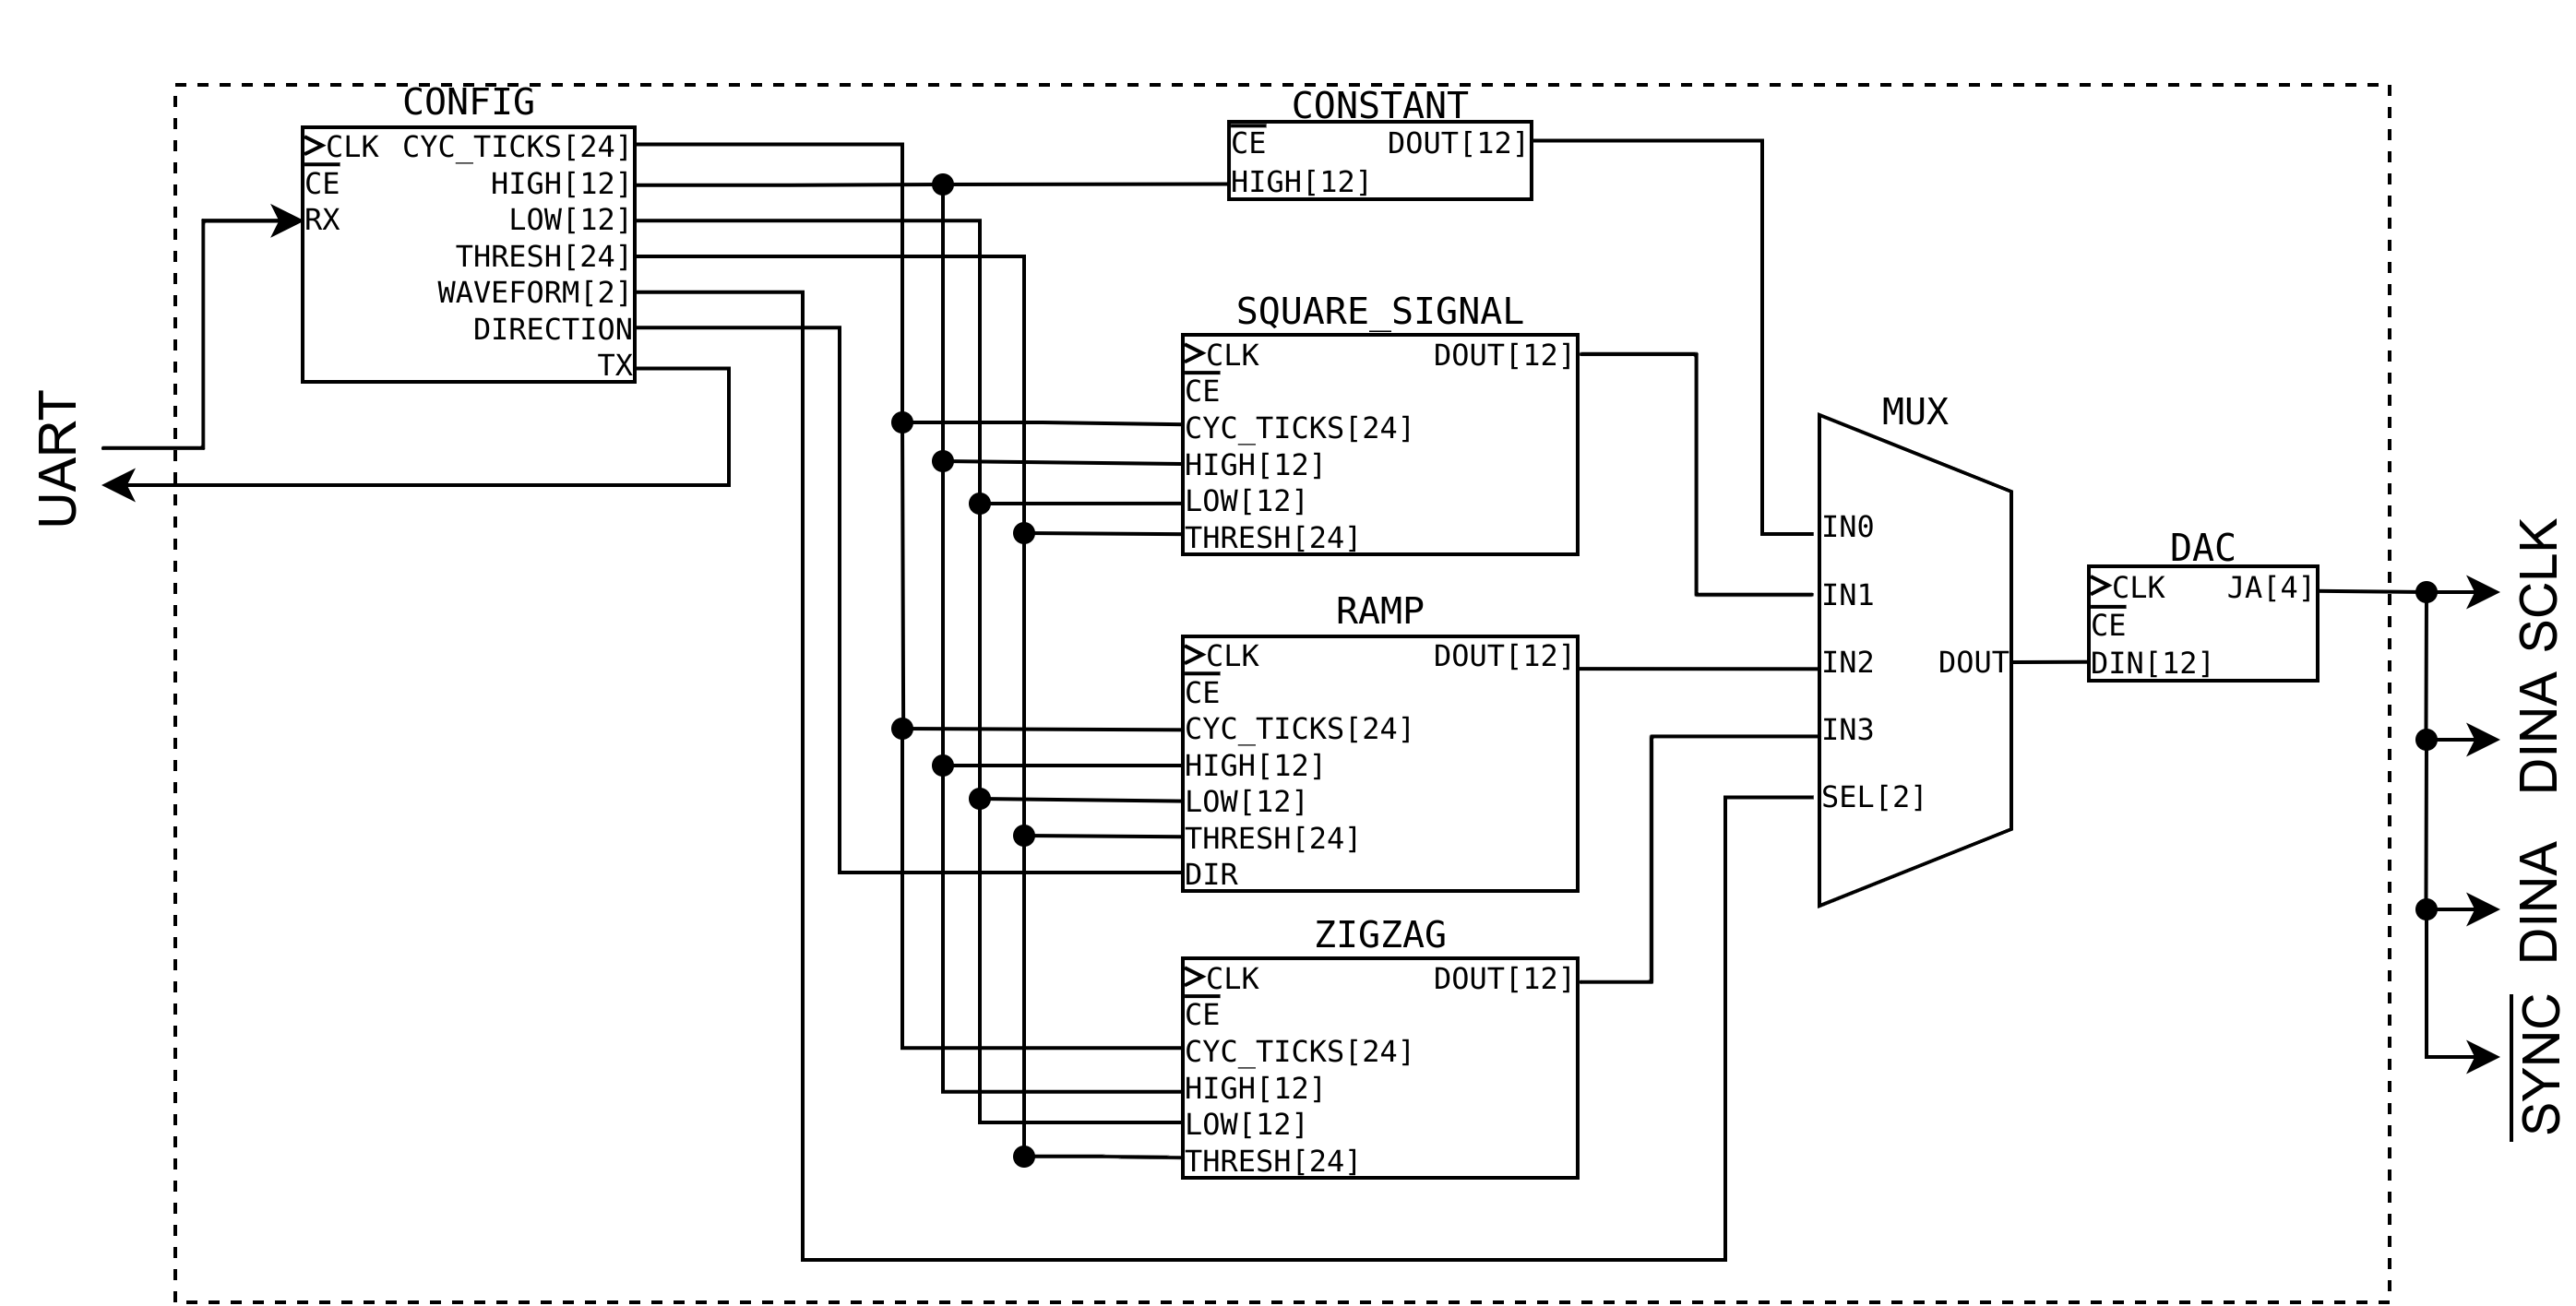
\includegraphics[width=1.0\textwidth, angle=-90, origin=c]{function_generator}
  \caption{Diagramm des Funktionsgenerators. Aus Gründen der Übersichtlichkeit sind die \bit{CLK} Signale und \lowactive{CE} Signale nicht angeschlossen dargestellt. Alle \bit{CLK} Signale sind an den Systemtakt angeschlossen und alle \lowactive{CE} Signale liegen auf Masse.}  \label{Concept:FuncGenDia}
\end{figure}

 % Gesamtkomponente beschreiben
\chapter{Komponenten}
In diesem Kapitel soll der Aufbau des Funktionsgenerators anhand seiner
digitaltechnischen Komponenten erläutert werden.

\section{Arithmetik}
Der Funktionsgenerator braucht für die richtige Berechnung des Ergebnisses Komponenten, mit deren Hilfe mathematische Operationen ausgeführt werden können.
Zum Addieren, Subtrahieren und Multiplizieren vorzeichenloser Zahlen können die VHDL Standardfunktionen des Datentyps \code{unsigned} verwendet werden.
Darüber hinaus benötigte Funktionen, die über eine eigene Implementierung verfügen, werden im Folgenden vorgestellt.

\subsection{Zähler} \label{Comp:Arith:Count}
Der Zähler bildet die Basiskomponente der Funktionskomponenten. Er eignet sich sehr gut, um die Zeit zu messen, da sich die Zeit seit dem letzten Rücksetzen des Zählers $T_{R}$ immer aus dem Zählstand $N$ und der Taktzeit des Zählers $T_{count}$ berechnen lässt: $T_{R} = N \cdot T_{count}$. So kann durch wiederholtes Rücksetzen des Zählers bei einem bestimmten Zählstand ein zyklischer Funktionsverlauf erstellt werden.
Der Zählstand selbst dient in diesem Fall als diskrete X-Komponente, der dann von der Funktionskomponente ein Y-Wert zugeordnet wird.
Der hier implementierte Zähler kann allerdings schon selbst als Funktionskomponente mit dem Ausgang $o\_count$ für die Funktion $o\_count = inc \cdot N \cdot (-1) ^ {1 - D}, N \in \{0, 1, 2, \dots, max\_ticks\}$ gesehen werden.
Die Komponente besitzt nämlich die Eingänge \code{inc}, \code{D} und \code{max\_ticks}. Diese erfüllen folgende Aufgabe:
\begin{itemize}
\item \code{max\_ticks}: Bit-Vektor, der den maximalen Wert repräsentiert, ab dem der Zähler automatisch zurückgesetzt wird.
Diese Funktion erleichtert es, die Zykluszeit einer Funktion $T_{func}$ als Zeitraum zwischen zwei Rücksetzungen festzulegen: $T_{func} = max_{ticks} \cdot T_{func}$
\item \code{D}: Richtung, in die der Zähler Zählen soll: 0 heißt aufwärts, 1 heißt abwärts
  \item \code{inc}: Bit-Vektor, er repräsentiert das Inkrement, um das der Zähler hoch- bzw. runterzählen soll
\end{itemize}

Der maximale Zählstand ist durch die Anzahl der Stellen von \code{o\_count} beschränkt. Sie kann generisch durch den Wert \code{data\_width} bestimmt werden. \\
Würde es im nächsten Takt dazu kommen, dass der Zählstand größer als \code{max\_ticks} wird (Überlauf), setzt er sich automatisch wieder auf Null zurück.
Würde es im nächsten Takt dazu kommen, dass der Zählstand kleiner als Null wird (Unterlauf), wird der Zähler auf \code{max\_ticks} zurückgesetzt.
Zusätzlich kann der Zähler asynchron auf Null gesetzt werden, wenn der Eingang \code{R} auf 0 gesetzt wird.


\subsection{Teiler} \label{Comp:Arith:Division}
Während beim Multiplizieren, Addieren und Subtrahieren auf Standardfunktionen
zurückgegriffen wird, wird für die Division zweier Binärzahlen eine eigene
Komponente entworfen. Die Gründe hierfür werden in \cref{Comp:Func:ZigZag}
erläutert. \\ % Quelle: https://en.wikipedia.org/wiki/Division_algorithm
Diese Komponente kann die Division des Zählers $Z$ durch den Nenner $N$
lösen, dabei sind $Z$ und $N$ zwei Binärzahlen mit gleicher
Stellenanzahl und ohne Vorzeichen. Das Ergebnis ist der Quotient $Q$ und der Rest $R$. Der Algorithmus, den die Komponente ausführt, ermittelt dabei pro Rechenschritt (d.h. pro Takt) eine Stelle des Ergebnisses.
Er geht den Zähler von der größten bis zur kleinsten Stelle durch und schiebt die immer die aktuelle Stelle $Z(i)$ in den Rest, sodass der neue Rest im binären $R' = R \cdot 2 + Z(i)$ ist.
Immer wenn der Rest größer wird als der Nenner, ist das Ergebnis der Division größer Null, also wird der neue Rest durch Subtraktion mit dem Nenner gebildet: $R'' = R' - N$.
Ist eine Subtraktion möglich, ist $Q$ an dieser Stelle Eins, ansonsten ist $Q$ Null. Der nachfolgende Pseudocode verdeutlicht den Algorithmus noch einmal.
Es gilt dabei aber zu beachten, dass alle Schritte innerhalb der Schleife in einem Takt ausgeführt werden können, da es sich bei der Komponente um eine digitale Schaltung handelt.

\begin{verbatim}
Beginn des Algorithmus
// verhindern, dass durch 0 geteilt wird:
wenn N ungleich 0, dann
    setze Q = 0
    setze R = 0
    zähle i von n - 1 bis 0 runter  // n ist die Anzahl der Bits in N
        schiebe R um 1 Bit nach links
        // letzte Stelle von R wird ite Stelle des Zählers:
        R(0) = Z(i)                    
        wenn R >= N, dann               
            setze R = R - N
            setze Q(i) = 1  // ite Stelle des Quotienten wird 1 
        Ende der bedingten Anweisung
    springe zum Anfang der Schleife
Ende der bedingten Anweisung
Ende des Algorithmus
\end{verbatim}

\section{Takterzeugung}
Da die Einzelkomponenten des Funktionsgenerators in verschiedenen Geschwindigkeiten arbeiten, braucht es Komponenten für das Clock-Management. 
\subsection{Clock-Enable} \label{Comp:Tact:ClkEn}
Um aus dem Systemtakt Takte mit niedrigerer Frequenz zu erzeugen, wird die Komponente \code{SCLK\_ENABLE} verwendet.
Der Takt wird geteilt, indem ein sogenanntes Enable-Signal \code{SCLK\_EN} erzeugt wird, das die jeweils nte steigende Flanke des Systemtakts mit \code{low} maskiert.
Der Eingang \code{CE} der Komponente, die im erzeugten Takt arbeiten soll, wird an \code{SCLK\_EN} angeschlossen, so dass die Komponente nur dann aktiv ist, wenn eine steigende Flanke detektiert wurde und \code{CE=0} anliegt.
Das Timingdiagram in Abbildung \cref{Comp:Tact:ClkEn:Timing} verdeutlicht, auf welche Taktzyklen die angeschlossene Komponente reagiert.
Der große Vorteil dieser Methode liegt darin, dass jede Komponente weiterhin direkt an den Systemtakt angeschlossen ist und dieser somit nicht durch zwischengeschaltete Komponenten verzögert wird.
\vfill
\begin{tikztimingtable} 
  CLK                             & H 9{2L 2H} L    \\
  $\overline{\mbox{CLK\_Enable}}$ & H 3{4L 8H} L    \\
  aktive Zyklen                   & 3L 3{2H 10L} L  \\
  \extracode
  \tablerules
  \begin{pgfonlayer}{background}
    \foreach \n in {1, ..., 8}
    \draw [help lines] (A\n) -- (B\n);
  \end{pgfonlayer}

\end{tikztimingtable}
\captionof{tikztimingtable}{Beispielhaftes Timing-Diagramm. Jeder vierte Taktzyklus wird durch \lowactive{CLK\_Enable} aktiviert.} \label{Comp:Tact:ClkEn:Timing}


\section{Funktionen}   \label{Comp:Func}
Die Herzstücke des Funktionsgenerators bilden seine Funktionskomponenten.
An ihren Ausgängen liegen die von ihnen berechneten Werte an, von denen einer zum in \cref{Comp:DAC} beschriebenen DAC-Konverter per Multiplexer weitergeleitet wird.
Bis auf die Konstante verfügen alle Komponenten, neben den üblichen \code{CLK} und \lowactive{CE} Eingängen, über folgende Anschlüsse:

\begin{itemize}
\item \code{cyc\_ticks}: Eingang, dieser Bit-Vektor legt die Periodendauer einer Funktionskomponente fest.
\item \code{high}: Eingang, dieser Bit-Vektor legt den maximal erreichbaren Wert des Komponentenausgangs fest.
\item \code{y\_out}: Ausgang, der digitale Funktionswert, der zum DAC geschickt wird
\end{itemize}

Alle Komponenten außer der Konstante verfügen über einen Zähler und eine Clock-Enable-Komponente, die die Geschwindigkeit des Zählers steuert.
Darüber hinaus können sie noch über drei generische Größen konfiguriert werden:

\begin{itemize}
\item \code{data\_width}: legt die Bitbreite des \code{high}, \code{low} und \code{y\_out} Signals fest.
Bei allen Funktionen ist diese auf zwölf eingestellt, da es sich beim DAC-Wandler um einen 12-Bit-Konverter handelt.
\item \code{clk\_width}: legt die Bitbreite von \code{cyc\_ticks} und \code{thresh} fest.
  Diese muss größer als \code{data\_width} sein.
  Die \code{clk\_width} legt fest, welche Periodendauer maximal erreicht werden kann, da sie den maximal möglichen Zählerstand begrenzt.
\item \code{clk\_ticks\_per\_count}: Dies ist der Teilungsfaktor zwischen dem angelegten Takt und dem Takt, mit dem der interne Zähler hochzählt.
\end{itemize}


\subsection{Konstante}   \label{Comp:Func:Const}
Die konstante Funktion ist die einfachste der vier Funktionskomponenten.
Sie gibt lediglich den an ihr anliegenden high-Wert auf ihrem Ausgang aus.
Sie verfügt darüber hinaus noch über den Eingang \lowactive{CE}, der bewirkt, dass der Ausgang asynchron auf 0 gesetzt wird.
\subsection{Rechteck}   \label{Comp:Func:Square}
Die Rechteckfunktion verfügt über einen Eingang \code{thresh}, der mit dem Stand des internen Zählers verglichen wird.
Ist der Zähler größer als \code{thresh}, so wird der Ausgang auf den Wert \code{high} gesetzt, ansonsten ist er auf den Wert \code{low} eingestellt.
Der \code{low}-Wert liegt als weiteres Eingangssignal an.

\subsection{Zick-Zack}  \label{Comp:Func:ZigZag}


\subsection{Rampe} \label{Comp:Func:Ramp}

\section{Konfigurationsschnittstelle}
Die Konfigurationsschnittstelle \code{CONFIG\_INTERFACE} besteht aus einer
UART-Schnittstelle, über die der Datenaustausch zwischen Benutzer und
Funktionsgenerator erfolgt, sowie der Instruktionsauswertung, die die
empfangenen UART-Signale in Konfigurationsbefehle übersetzt.
\subsection{UART-Schnittstelle}
Die UART-Schnittstelle beruht auf dem
\textbf{U}niversal-\textbf{A}synchronous-\textbf{R}ceiver-\textbf{T}ransmission-Protokoll.
Das Protokoll ermöglicht es, byteweise serielle Daten zu verschicken und zu
empfangen. Hierfür reichen zwei Drähte aus, die jeweils eins der beiden Signale
RX (Receive) und TX (Transmit) transportieren. Zum Start der Kommunikation wird
die RX Leitung vom Sender von high auf low gezogen. Der Empfänger detektiert
dieses Startsignal und fängt an, die nachfolgenden acht Bits zu einem Byte
zusammenzusetzen.
Wurde ein Byte übertragen, muss mindestens ein Stop-Bit folgen, bei dem die Receive Leitung des Empfängers auf
High liegt. Darauf kann, je nach Implementierung, noch ein Stop-Bit sowie
ein Paritätsbit folgen. Da es zwischen dem Sender und Empfänger kein synchrones
Taktsignal gibt, ist es wichtig, dass ihre Sende- und Empfangsfrequenz gleich
ist. Diese Frequenz ist die sogenannte Baudrate. Im Funktionsgenerator ist sie
auf 115200 Bits / s festgelegt. \\
Die im Generator verwendete Schnittstelle wurde,
um den Arbeitsaufwand zu verringern, aus einer Vorlage übernommen (Quelle). Sie
beinhaltet sowohl eine Empfänger- als auch eine Sender-Komponente. Es gibt
folgende Eingangssignale:
\begin{enumerate}
\item \code{CLK}: Eingang, gibt die Taktfrequenz der Komponente vor
\item \code{CE}: Eingang, ''chip-enable``-Signal, aktiviert die Komponente wenn es auf
  low gesetzt wird
\item \code{reset}: Eingang, die Schnittstelle wird auf den Initialisierungszustand zurückgesetzt und die aktuelle Übertragung bzw. aktuelle Empfangsprozesse werden abgebrochen.

\item \code{tx}: Ausgang, Das von der Schnittstelle versendete TX-Signal 
  \item \code{tx\_start}: Eingang, wenn \code{tx\_start} auf high gesetzt wird, wird mit der
    Übertragung von \code{data\_in} begonnen
\item \code{data\_in}: Eingang, ein 8-Bit breites Signal, dass das zu versendende Byte enthält.

\item \code{rx}: Eingang, das von der Schnittstelle empfangene RX-Signal
\item \code{data\_out}: Ausgang, ein 8-Bit breites Signal, dass das zuletzt von der Schnittstelle empfangene Byte beinhaltet.
\item \code{rx\_uart\_rdy}: Ausgang, dieses Signal zeigt an, wenn ein komplettes Byte
  empfangen wurde und bereit ist, gelesen zu werden.
\end{enumerate}
  
\subsection{Instruktionsauswertung}

\section{DAC-Konverter} \label{Comp:DAC}
\subsection{DAC-Kanal}

 % Einzelkomponenten beschreiben
\chapter{Funktionstest}
Nach der Implementierung des zuvor geschilderten Konzepts wird ein Funktionstest durchgeführt.
Dazu werden zunächst die theoretischen Grenzen der Konfiguration getestet und danach die tatsächlichen Ausgabewerte mit den theoretischen verglichen.
Besonders interessant ist hierbei, in welchem Frequenzbereich der Generator zuverlässig funktioniert.

\section{theoretische Limitierungen}
Um den praktischen Nutzen des Funktionsgenerators einzuschätzen, werden die Grenzen der einstellbaren Frequenz, die Auflösung und der Spannungsbereich berechnet.
Für die Spannung ergeben sich diese Werte aus dem Datenblatt des eingesetzten DACs.
Dieser kann in einem Bereich von 0 bis 5,5 V eingesetzt werden, wobei die Referenzspannung 2,7 V nicht unterschreiten darf \cite{PmodDA2}.
Für den Betrieb auf dem Basys 3-Board läuft der Spannungsbereich von 0 bis 3,3 V, da hier die Ausgangsspannung des Boards der limitierende Faktor ist.
Nachfolgend werden noch der Frequenzbereich und die Auflösung bestimmt.

\subsection{Frequenzbereich}
Der Systemtakt $f_{sys}$ des Generators beträgt 100 MHz.
Der Frequenzbereich der Funktionen, die er ausgeben kann, reicht von ca. 0,0877 Hz bis zu ca. 735 kHz für die Rampen- und Rechteckfunktion.
Für die Zick-Zack-Funktion beträgt $f_{max}$ nur die Hälfte, also ca. 365 kHz.\\

\begin{align}
  f_{count} &= \frac{f_{sys}}{68} \label{test:theo:freq:fcount}\\  
  f_{max} &= \frac{f_{count}}{2}  \label{test:theo:freq:fmax}\\ 
  f_{min} &= \frac{f_{count}}{2^{clk\_width} - 1} \label{test:theo:freq:fmin}
\end{align}

Die Frequenz $f_{count}$ ist die Frequenz mit der der interne Zähler der Funktionsbausteine hochzählt.
Er beträgt ein 68tel des Systemtakts $f_{sys}$ (siehe \cref{test:theo:freq:fcount}).
Die minimale Frequenz $f_{min}$ errechnet sich aus dem maximalen Zählstand, der wiederum abhängig ist von seiner Bitbreite \code{clk\_width} (siehe \cref{test:theo:freq:fmin}).
Die maximale Frequenz ergibt sich aus dem Shannon'schen Abtasttheorem, nach dem die minimale Abtastfrequenz eines Signals doppelt so groß sein muss, wie die Frequenz des abgetasteten Signals.
In diesem Fall entspricht die Abtastfrequenz $f_{count}$ und das abgetastete Signal dem Ausgangssignal, woraus folgt, dass das ausgehende Signal nur halb so groß sein kann, wie $f_{count}$ \cite{nyquist1928}. Damit berechnet sich $f_{max}$ nach \cref{test:theo:freq:fmax}.


\subsection{Auflösung}
Die Auflösung des analogen Ausgangssignals hängt sowohl von der Geschwindigkeit ab, mit der das digitale Signal analogisiert werden kann, als auch von der maximalen Anzahl digital darstellbarer Werte.
Überschreitet die Frequenz des analogen Signals $f$ die Grenzfrequenz $f_{grenz}$, so fällt die Auflösung $R$ reziprok zu $f$ ab (siehe \cref{test:theo:res:plot}).
Oberhalb von $f_{grenz}$ ist die Auflösung durch die Bitbreite des ADCs begrenzt.
Da es sich um einen 12-Bit Wandler handelt, beträgt die Anzahl darstellbarer Werte und damit auch die höchste Auflösung $2^{12} - 1 = 4095$.
Diesen Wert nimmt die Auflösung an, wenn die Frequenz kleiner als $f_{grenz}$ ist (siehe \cref{test:theo:freq:fgrenz}).

\begin{align}
  R &= \begin{cases}
    4095               & f \leq f_{grenz}                      \\
    \frac{f_{count}}{f} & f > f_{grenz} = \frac{f_{count}}{4095} = 359 Hz
        \end{cases} \label{test:theo:freq:fgrenz}
\end{align}

Konkret bedeutet dass für den Funktionsgenerator, dass bei einer Amplitude von $U_{SS}=3,3V$ und einer Frequenz von $f=100kHz$, die Auflösung $4,54V^{-1}$ statt der maximalen Auflösung von $1241V^{-1}$ beträgt, das heißt, dass bei 100kHz 4,54 Werte statt 1241 Werte pro Volt gesampelt werden.

\begin{figure}[h] \centering
    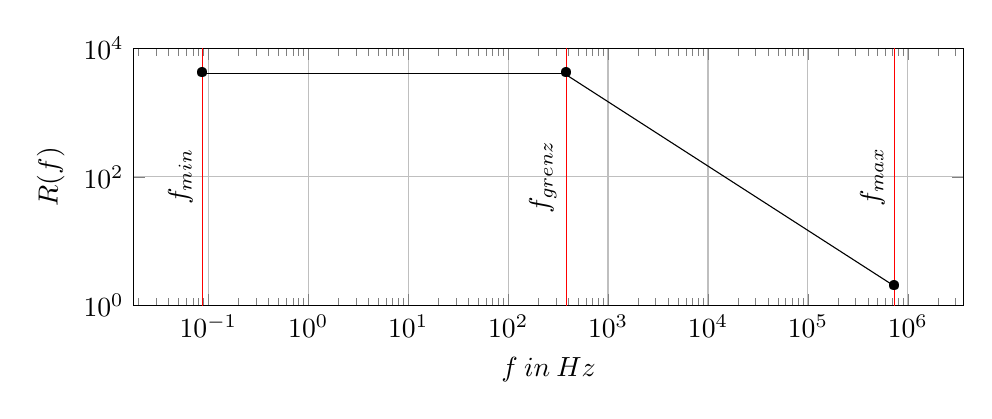
\begin{tikzpicture}
      \begin{loglogaxis}
        [xlabel=$f\:in\:Hz$,
        ylabel=$R(f)$,
        ymin=1,
        ymax=10000,,
        width=\textwidth,
        height=0.4\textwidth,
        grid=major]
        \addplot[color=black, domain=0.08765:359.12] {4095};
        \addplot[color=black, domain=359.12:735294] {100000000 / (68*\x)};
        % help lines and nodes:
        \addplot[color=red] coordinates{(381.12, 1)(381.12, 10000)};
        \node[above, rotate=90] at (381.12, 100) {$f_{grenz}$};
        \node at (381.12, 4095) {\textbullet};

        \addplot[color=red] coordinates{(0.08765, 1)(0.08765, 10000)};
        \node[above, rotate=90] at (0.08765, 100) {$f_{min}$};
        \node at (0.08765, 4095) {\textbullet};

        \addplot[color=red] coordinates{(735294, 1)(735294, 10000)};
        \node[above, rotate=90] at (735294, 100) {$f_{max}$};
        \node at (735294, 2) {\textbullet};
      \end{loglogaxis}
    \end{tikzpicture}
 \caption{Doppelt logarithmisches Diagramm der Auflösung $R(f)$ über den Frequenzbereich $f$. Die Auflösung bleibt konstant bei 4095 1/tick bis sie schließlich bei $f_{grenz}$ anfängt zu sinken.} \label{test:theo:res:plot}
\end{figure}

\section{reales Verhalten}
Nun soll das reale Verhalten des Funktionsgenerators untersucht werden.
Die dazu durchgeführten Versuche sind nachfolgend geschildert.

\subsection{Versuchsaufbau}
Ein Foto des Versuchsaufbaus findet sich in \cref{test:real:setup:pic}.
Das digitale Oszilloskop Analog Discovery 2 von digilent wird an einen Laptop angeschlossen, auf dem dann die Funktionsverläufe mit der Software digilent WaveForms angezeigt werden.

\begin{figure}[h] \centering
  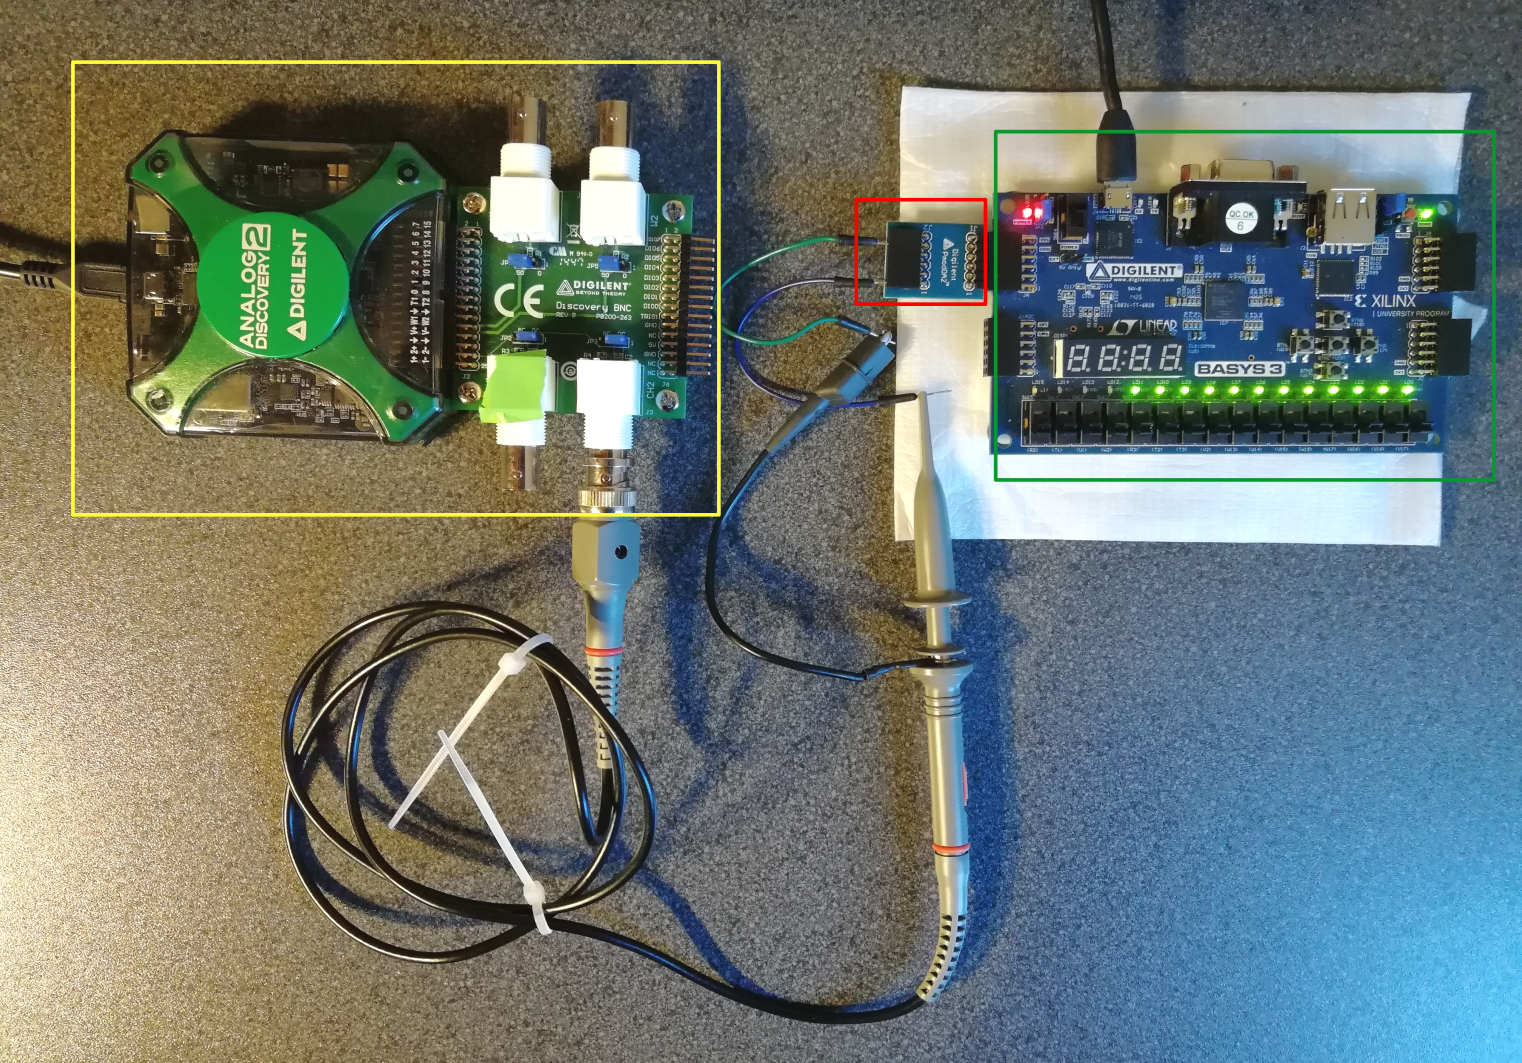
\includegraphics[width=0.8\textwidth]{testaufbau_annotated_fg}
  \caption{Versuchsaufbau zum Testen des Funktionsgenerators. Das Oszilloskop ist mittels des Discovery BNC Moduls (beide gelb umrandet) an den analog Ausgang des PmodDA2-Wandlers (rot umrandet) angeschlossen. Das Basys 3-Board (grün umrandet) wird über das angeschlossene USB Kabel mit Strom versorgt und per UART konfiguriert. Die vom Oszilloskop eingelesenen Daten werden an einen per USB angeschlossenen Laptop (nicht im Bild) verschickt. Die LEDs auf dem Board zeigen den internen digitalen Funktionswert an.}
  \label{test:real:setup:pic}
\end{figure}

\subsection{Versuchsdurchführung}
Um zunächst die korrekte Ausgabe der Funktionsverläufe zu überprüfen, werden alle vier Verläufe nacheinander bei konstanter Frequenz $f=100Hz$ über die UART-Schnittstelle konfiguriert und die erfassten Signale dokumentiert.
Der eingestellte \analog{low} und \analog{high} Wert beträgt 0 bzw. 3,3 V.\\
Anschließend werden alle Funktionen der UART-Schnittstelle überprüft, indem der jeweilige Befehl mit einem dazu passenden Argument abgeschickt wird. \\
Schließlich wird noch der Frequenzbereich anhand der Zick-Zack-Funktion untersucht.
Dazu wird ein Wert knapp unterhalb von $f_{min}$, ($f = 0,08Hz$), und ein Wert oberhalb von $f_{max}$, ($f = 1MHz$), eingestellt.
Dazwischen wird, von 0.1 Hz aufwärts, mit jedem Schritt die eingestellte Frequenz mit 10 multipliziert.
Die Werte für \analog{low} und \analog{high} werden wieder auf 0 und 3,3 V gesetzt.
Auffäligkeiten im Funktionsverlauf werden festgehalten und die Daten werden dann noch im CSV Format für weitere Auswertungen abgespeichert. \\
Um die Frequenz der Zick-Zack Funktion zu messen, werden alle Datenpunkte mitAusgangsspannung $U < 0,5 V$ betrachtet.
Aus den Zeitkomponenten nahe beieinander liegender Punkte wird dann der Mittelwert gebildet.
Die Differenz zweier aufeinanderfolgender Mittelwerte kann als Näherung für die Zykluszeit $T$ betrachtet werden, aus der dann die Frequenz des Signals mit $f = 1 / T$ berechnet wird.

\subsection{Ergebnis}

Zunächst werden Funktionsverläufe bei 100 Hz präsentiert (siehe \cref{test:real:res:plot}).

\begin{figure}[h] \centering
  {
    \pgfplotsset{
    no markers,
    grid=major,
    ymin=-0.2, ymax=3.5,
    scaled x ticks=false,
    ytick={0, 0.55, 1.1, 1.65, 2.2, 2.75, 3.3},
    xtick={-0.005, -0.0025, 0, 0.0025, 0.005},
    xticklabels={-5, -2.5, 0, 2.5, 5},
    width=0.45\textwidth}
  % constant
  \subfloat[][konstante Funktion]{ 
    \begin{tikzpicture}
      \begin{axis}[ylabel=$U(t)$ in V]
        \addplot table [x=Time (s), y=Channel 2 (V), col sep=comma, row sep=newline] {test/const100Hz_small.csv};
      \end{axis}
    \end{tikzpicture}
    \label{test:real:res:plot:const}
  } 
  % square
  \subfloat[][Rechteckfunktion]{
    \begin{tikzpicture}
      \begin{axis}
        \addplot table [x=Time (s), y=Channel 2 (V), col sep=comma, row sep=newline] {test/square100Hz_small.csv};
      \end{axis}
    \end{tikzpicture}
    \label{test:real:res:plot:square}
  } 

  % zigzag 
  \subfloat[][Zick-Zack-Funktion]{
    \begin{tikzpicture}
      \begin{axis}[ylabel=$U(t)$ in V, xlabel=$t$ in ms]
        \addplot table [x=Time (s), y=Channel 2 (V), col sep=comma, row sep=newline] {test/zigzag100Hz_small.csv};
      \end{axis}
    \end{tikzpicture}
    \label{test:real:res:plot:zigzag}
  }
  % ramp
  \subfloat[][Rampenfunktion]{
    \begin{tikzpicture}
      \begin{axis}[xlabel=$t$ in ms]
        \addplot table [x=Time (s), y=Channel 2 (V), col sep=comma, row sep=newline] {test/ramp100Hz_small.csv};
      \end{axis}
    \end{tikzpicture}
    \label{test:real:res:plot:ramp}
  }
}
\caption{Die Ergebnisse des Versuchs bei $f=100Hz$. Die konstante Funktion und die Rechteckfunktion weisen ein leichtes Rauschen auf. Ihr \analog{low} und \analog{high} Wert liegen dauerhaft unter 0 bzw. 3,3 V.} \label{test:real:res:plot}
\end{figure}

Die Verläufe bei $f = 100Hz$ ergaben sich auf den ersten Blick wie erwartet.
Ihre Frequenz wurde mit dem Cursor-Tool der Oszilloskop Software gemessen und ergab ca. 100 Hz.
Jedoch fiel auf, dass \analog{low} und \analog{high} nicht genau 0 bzw. 3,3 V betrugen.
Der Mittelwert des konstanten Signals betrug $\overline{U}_{c}=3,24 V$, beim Rechtecksignal lag der tiefste Wert bei $U_{sl} = -0,11 V$ und der höchste bei $U_{sh} = 3,25 V$, beim Zick-Zack-Signal waren es $U_{zzl} = -0,06 V$ und $U_{zzh} = 3,26 V$ und beim Rampensignal $U_{rl} = -0,1 V$ und $U_{rh} = 3,24 V$. \\
Der Generator ließ sich problemlos per UART konfigurieren.
Alle eingegebenen Befehle führten zu der erwarteten Ausgabe am analogen Ausgang.\\
Beim Abtasten der Frequenz  ergab sich bei Unterschreiten von $f_{min}$ ($f = 0,08Hz$) eine wesentlich höhere Frequenz von 20,5 Hz. 
Im niedrigen Frequenzbereich konnten nur geringe Abweichungen von der eingestellten Frequenz gemessen werden. \\
Je näher $f$ jedoch $f_{max}$ kam, desto stärker wich die gemessene Frequenz $f_{ist}$ von der eingestellten Frequenz $f_{soll}$ ab.
Die Messergebnisse der Frequenzmessung finden sich in \cref{test:real:res:ftab}.

\begin{table}[h]
  \begin{tabular}[h]{|l|r|r|r|r|r|r|r|r|r|r|}
    \hline
    $f_{soll}$ & 0,08 & 0,1 & 1 & 10 & 100 & $10^3$ & $10^4$ & $10^5$ & $3,5 \cdot 10^5$ & $10^6$\\ \hline
    $f_{ist}$ & 20,5 & 0,100 & 1,01& 10,1 & 101 & 999 & $10^4$ & $9,81 \cdot 10^4$ & $2,94 \cdot 10^5$ & - \\ \hline
  \end{tabular}
  \caption{Diese Tabelle stellt die eingestellten Frequenzen $f_{soll}$ in Hz den gemessenen Frequenzen $f_{ist}$ in Hz gegenüber. Für $f_{soll} = 10^6 Hz$ konnte die Frequenz nicht bestimmt werden.} \label{test:real:res:ftab}
\end{table}

Die Verläufe ab einer Frequenz $f > 10 kHz$ wiesen starke Schwankungen auf, die zu einem unsauberen Signal führten (siehe \cref{test:real:res:zzplot}).
Je näher die Frequenz $f_{max}$ kam, desto deutlicher wurde die begrenzte Auflösung, wie in \cref{test:real:res:zzplot:350kHz} zu sehen ist.
Außerdem ändert sich der Wert nicht sprunghaft, sondern eher entsprechend der Ladekurve eines Kondensators.

\begin{figure}[h] \centering
  {
    \pgfplotsset{
    no markers,
    grid=major,
    ymin=-0.2, ymax=3.5,
    scaled x ticks=false,
    ytick={0, 0.55, 1.1, 1.65, 2.2, 2.75, 3.3},
    yticklabels={},
    width=0.37\textwidth}
  \subfloat[][10 kHz]{ 
    \begin{tikzpicture}
      \begin{axis}[ylabel=$U(t)$ in V, xlabel=$t$ in µs,
                   xtick={-0.000075, -0.00005, -0.000025, 0, 0.000025, 0.00005, 0.000075},
                   xticklabels={, -50, , 0, , 50,},
                   yticklabels={0, , 1.1, , 2.2, , 3.3}]
        \addplot table [x=Time (s), y=Channel 2 (V), col sep=comma, row sep=newline] {test/zigzag10000Hz_small.csv};
      \end{axis}
    \end{tikzpicture}
    \label{test:real:res:zzplot:10kHz}
  } 
  \subfloat[][100 kHz]{
    \begin{tikzpicture}
      \begin{axis}[xlabel=$t$ in µs,
        xtick={-0.0000075, -0.000005, -0.0000025, 0, 0.0000025, 0.000005, 0.0000075, 0.000010},
                   xticklabels={, -5, , 0, , 5, , 10}]
        \addplot table [x=Time (s), y=Channel 2 (V), col sep=comma, row sep=newline] {test/zigzag100000Hz_1cyc.csv};
      \end{axis}
    \end{tikzpicture}
    \label{test:real:res:zzplot:100kHz}
  } 
  \subfloat[][350 kHz]{
    \begin{tikzpicture}
      \begin{axis}[xlabel=$t$ in µs,
                   xtick={-0.000004, -0.000002, 0, 0.000002, 0.000004},
                   xticklabels={-4, -2, 0, 2, 4}]
        \addplot table [x=Time (s), y=Channel 2 (V), col sep=comma, row sep=newline] {test/zigzag350000Hz_1cyc.csv};
      \end{axis}
    \end{tikzpicture}
    \label{test:real:res:zzplot:350kHz}
  }
}
  \caption{Signalverläufe ab 10 kHz. Während in \cref{test:real:res:zzplot:10kHz} das Signal noch gut zu erkennen ist, ist es in \cref{test:real:res:zzplot:100kHz} schon sehr undeutlich. In \cref{test:real:res:zzplot:350kHz} liegt die Frequenz schließlich so nah bei $f_{max}$, dass die Auflösung von 4 Schritten erkennbar wird.} \label{test:real:res:zzplot}
\end{figure}

\subsection{Auswertung}
Der Funktionsgenerator gibt die per UART konfigurierten Signale korrekt aus. 
Allerdings scheinen, auch durch den DAC-Konverter, die Genauigkeit und die Bandbreite beschränkt zu sein. \\
Die ungenaue Ausgabe der Spannungswerte \analog{high} und \analog{low} könnte daher kommen, dass der Chip die Versorgungsspannung des Basys 3 Boards als Referenzspannung nutzt.
Da aber mehrere Verbraucher und der Chip selsbt von dieser Spannung gespeist werden, kann sie schnell ungenau werden.
Ein anderer Chip mit einem weiteren Pin für eine Referenzspannung könnte die Genauigkeit erhöhen.
Für einfache Signalverläufe ist sie aber ausreichend. \\
Stellt man die Frequenz auf $f < f_{min}$ ein, so stellt man fest, dass eine größere Frequenz als $f_{min}$ ausgegeben wird.
Dies ist damit zu erklären, dass der interne Zähler eine beschränkte Breite von 24 Bit hat.
Damit beträgt sein maximaler Wert $2^{24} - 1 = 16.777.215$.
Vom Konfigurationswert werden nur die letzten 24 Stellen übernommen, sodass sich der interne Wert wiederum kleiner als $2^{24} - 1$ ist.
Daraus resultiert eine höhere Frequenz als der Nutzer konfigurieren wollte.\\
Die Frequenz zeigt sich bis $f = 10^4 Hz$ stabil, jedoch wird sie zu $f_{max}$ hin sehr ungenau.
Dies ist auf die begrenzte Geschwindigkeit des Zählers der Funktionsbausteine zurückzuführen.
Es können nur Zykluszeiten eingestellt werden, die Vielfache der Zählerzykluszeit sind.
Dieser Umstand fällt dann stärker ins Gewicht, wenn es nur wenige Zyklen abzuzählen gibt, was bei sehr hohen Frequenzen der Fall ist. \\
Auch der ungenaue Signalverlauf lässt sich teilweise mit der begrenzten Zähler-geschwindigkeit und der daraus resultierende sinkenden Auflösung erklären.
Jedoch hätte der Verlauf immer mehr die Form einer Treppe annehmen müssen, da die Auflösung mit steigender Frequenz abnimmt und die Änderung der Spannung pro Konvertierung größer wird.
Eine Ursache für dieses Verhalten kann nicht eindeutig bestimmt werden.
Es könnte daher kommen, dass der DAC-Konverter nicht ausreichend Zeit zur Konvertierung hat.
Andere Fehlerquellen könnten der Messaufbau oder ein Fehler beim versenden der Digitalwerte vom FPGA an den Konverter sein.
Weitere Untersuchungen, eventuell mit einem hochwertigeren Oszilloskop, könnten hier für Erkenntnis sorgen.
 % Kommt das raus was man einstellt? Für jede Waveform Frequenzbereich abgehen, theorie praxis vergleich
%Schluss
\chapter{Fazit}
Es wurde erfolgreich ein digitaler Funktionsgenerator auf dem Basys 3 Board implementiert.
Dieser kann vier verschiedene Funktionen ausgeben und über eine UART Schnittstelle konfiguriert werden. \\
Das dem Generator zugrundeliegende Konzept und das Zusammenspiel der Einzelkomponenten wurde erläutert.
Auch das interne Clock-Management wurde geschildert. \\
Die theoretischen Grenzen der Auflösung und der Frequenz wurden aufgezeigt. 
Darüber hinaus konnte seine Funktionstüchtigkeit in dem Frequenzbereich 0,1 Hz bis 10 kHz bewiesen werden.
Alle Frequenzen unterhalb von $f_{min}$ führen zu einer höheren Ausgangsfrequenz als der gewünschten.
Zwischen 10 kHz und $f_{max}$ wird das Ausgangssignal unsauber und oberhalb von $f_{max}$ ist eine zuverlässige Ausgabe nicht mehr möglich.
Warum das Signal oberhalb von 10 kHz derart ungenau wird, konnte teilweise erklärt werden.
Hier sollten jedoch weitere Untersuchungen angestrebt werden, um die Fehlerursache vollständig zu klären.\\
Die Ausgangsspannung entspricht nicht ganz der eingestellten Spannung.
Eine bessere Referenzspannung könnte aber für einen saubereren Ausgangspegel sorgen.
Allerdings wurde die Korrektheit des Ausgangspegels bis jetzt nur für die Spannung 0 und 3,3 V untersucht.
Um ein vollständigeres Bild der Genauigkeit zu bekommen, sind weitere Nachforschungen nötig.\\
Es wurde gezeigt, dass die Konfiguration per UART-Schnittstelle funktioniert.
Außerdem wurde der Befehlssatz des Funktionsgenerators dokumentiert, sodass andere.

\chapter{Ausblick}
Durch die Implementation der Funktionskomponenten als Bausteine ist es relativ leicht, die möglichen Funktionsformen zu erweitern.
Z.B. könnte noch eine Sinusfunktion hinzugefügt werden.
Theoretisch könnte auch ein nicht-periodisches Signal, wie ein zeitversetzter Sprung hinzugefügt werden.\\
Außerdem kann die UART-Schnittstelle noch um weitere Features ergänzt werden.
Es wäre beispielsweise denkbar, die gegenwärtigen Funktionsparameter über den Transmitter an den User zurück zu schicken, sodass dieser sie leichter kontrollieren kann.
Dazu müsste auch die Konfigurationsschnittstelle um Befehle zur Rückgabe der Funktionsparameter erweitert werden. \\
Darüber hinaus könnte auch noch der zweite Kanal auf dem DAC-Konverter genutzt werden um zwei verschiedene Signale gleichzeitig auszugeben. \\
Abschließend fehlt auch noch der Test in einer realen Anwendung, z.B. einem Trigger für eine Fotokamera, die in einer bestimmten Frequenz Bilder aufnehmen soll.

\end{document}
